\documentclass[10pt,onecolumn]{article}
\usepackage{graphicx}
\usepackage{hyperref}
\usepackage{url}
\usepackage{wrapfig}
\usepackage{listings}
\usepackage{tikz}
\usetikzlibrary{shapes}

\newcommand{\horrule}[1]{\rule{\linewidth}{#1}}

\title{\vspace{-4.2cm} \huge Project Report for Tracking Interconnected Facebook Links }
\author{ \horrule{1pt} \\ \textbf{ELEN4009 - Software Engineering} \\ \emph{University of the Witwatersrand} \\ \horrule{1pt} \\\\ \emph{Back-End Pair:} \\ Julian Zeegers (704582) \\ James Allingham (672732) \\ \\ \emph{Front-End Pair:} \\ Joseph Gage (751052)\\ Nathan Haag (873666) \\ \horrule{1pt}}

\addtolength{\oddsidemargin}{-1.5cm}
\addtolength{\evensidemargin}{-.0cm}
\addtolength{\textwidth}{3cm}


%%%%%%%%%%%%%%%%%%%%%%%%%%%%%%%%%%%%%%%%%%%%%%%%%%%%%%%%%%%%%%%%%%%%%%%%%%%%%%%
\begin{document}
\date{\vspace{-5ex}}
\maketitle
\pagestyle{plain}
\setcounter{page}{1}
\newpage

\section{Introduction}

	\subsection{Problem Statement} % James

	\subsection{Project Objectives} % James

	\subsection{Stakeholders} % James

	\subsection{Abbreviations} % All of us

\section{The Front-End}

	\subsection{Software Requirement Specification} % James

	\subsection{Design Document} % Joe
	This section was written in accordance with the IEEE Std 1016-1987 for Software Design Documents (SDD) \cite{IEEE}. 
	
	The section is divided into sub sections representing the different views of the design, namely the home page view, the friend network diagram view and the friend status word chart view.
		\begin{figure}
			\centering
			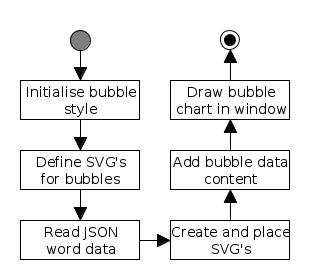
\includegraphics[scale=1]{bubbles}
			\caption{Code structure for bubble chart drawing script.}
		\end{figure}
		
		\begin{figure}
			\centering
			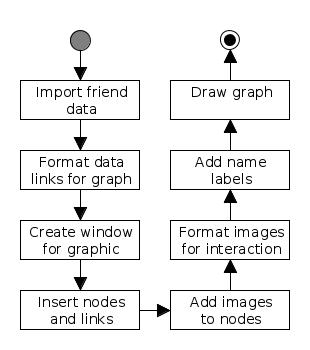
\includegraphics[scale=1]{network}
			\caption{Code structure for friend network drawing script.}
		\end{figure}

	\subsection{Implementation} % Nathan

\section{The Back-End}

	\subsection{Software Requirement Specification} % James

	\subsection{Design Document} % Joe
	This section was written in accordance with the IEEE Std 1016-1987 for Software Design Documents (SDD) \cite{IEEE}. 
	
	The back-end design consists of a graphical database system containing supporting functionality for making friend network queries as well as a web application framework. Both views were designed using a functional methodology. The particular functionalities of the design are documented below.
	
	The section is divided into sub sections representing the different views of the design, namely the database view and the web application framework view.
	
	\subsubsection{The Web Application Framework}
	This section will discuss the functions, dependencies and details of the web application framework. The general operation of the system is shown in Figure \ref{fig:django}.
	
		\begin{figure}[htb] 
			\centering
			
\includegraphics[scale=1]{django}
			\caption{Code structure for running of web application and processing user input.} \label{fig:django}
		\end{figure}
		
	The following functions were used in the web application framework: home, friendNetwork and wordChart. These functions refer to the different pages served by the web application. Each of these functions simply return the file path to the requested page which is the input to each function.
	
	The friendNetwork function, however, also calls a database supporting function to retrieve data which the page supported by the friendNetwork function requires. The function not only returns the file path but also the content for the page to use.
	
	The web application framework has the following dependencies: Django web framework, Apache HTTP server, Web Server Gateway Interface (WSGI), Python  and the page documents \cite{django, apache, wsgi}. Django was the framework used for integrating the source code used in the web application. Apache was the HTTP server used to host the web application. WSGI integrates the Django framework and the Apache server. Python was the programming language used by the framework. The page documents were stored within the Django framework and were required by the functions described above. 
	
	Several other details of the web framework are important. Firstly, the web application file system contains all of the dependencies of the functions mentioned as well as their supporting functions. Secondly, the file system also contains several configuration files specific to Django. Finally, several other scripts are required to run to start the server and web application - these are standardly available with the dependencies used.
	
	\subsubsection{The Graphical Database}
	This section will discuss the functions, dependencies and details of the the graphical database. The general operation of the supporting functions of the system is shown in Figure \ref{fig:db}.
	
		\begin{figure} [htb]
			\centering
			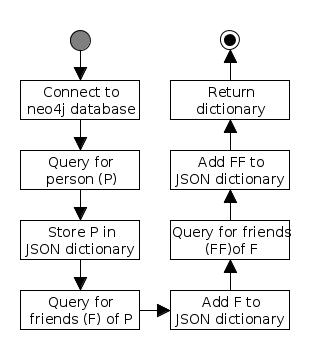
\includegraphics[scale=1]{neo4jdb}
			\caption{Code structure for fetching friends of friends network from neo4j DB.} \label{fig:db}
		\end{figure}

	The following functions were used to support the graphical database: getPerson, getFriendNetwork and getFoFNetwork. These functions each take as inputs the name and surname of the person being queried and return a dictionary containing the query results. 
	
	The getPerson function uses the name and surname input to query the database for the requested person. The function returns a dictionary containing the person in a node.
	
	The getFriendNetwork function uses the name and surname input to query the database for the requested person and the person's friends as well as the links between them. This function makes use of the getPerson function. The function returns a dictionary containing all of the queried persons in nodes and the relationships between them in links.
	
	The getFoFNetwork function uses the name and surname input to query the database for the requested person, the person's friends and the friends of the person's friends as well as the links between them. This function makes use of the getFriendNetwork function. The function returns a dictionary containing all of the queried persons in nodes and the relationships between them in links.
	
	The graphical database has the following dependencies: neo4j, py2neo and JSON \cite{neo4j, py2neo, JSON}. neo4j was the graphical database used in the software. py2neo was the Python API which was used in order to enable use of the database by the Python programming language. The web framework required use of Python. The dictionaries returned by the functions mentioned above were in JSON format.
	
	Two other details of the database are important. Firstly, the fields in the dictionaries returned by the above functions were nodes and links where each node and link had sub-fields. An example of their format is shown in Listing \ref{list:dbjson}. Secondly, the database requires an initialisation and migration to start it up. Standard code is provided for these functionalities.
	
	\begin{lstlisting}[caption=test,captionpos=b,label=list:dbjson]
		Please insert JSON dictionary example here Jamie!
	\end{lstlisting} 
		
	\subsection{Implementation} % Nathan

\section{Sprint Planning} % Julian

\section{Sprint Retrospective} % Julian

\begin{thebibliography}{1}
	\bibitem{IEEE} IEEE Standards Board. \emph{IEEE Guide to Software Design Descriptions}. IEEE, New York, 25 May 1993.
	\bibitem{Kinsey} H. van Vliet, \emph{Software Engineering: Principles and Practice} Wiley, 2007.
	\bibitem{twotieradvantage} N. Liyanage. \emph{Client/Server Architecture: Advantages and Disadvantages of the architectures}. 2013. \url{http://clientserverarch.blogspot.co.za/2013/03/advantages-and-disadvantages-of.html} Last accessed: 9 March 2016
	\bibitem{beginningsofteng} R. Stephens, Beginning Software Engineering, 1st ed. Indianapolis: John Wiley And Sons, Inc, 2015, pp. 94-95.
	\bibitem{Bootstrap}  \emph{Get Bootstrap - 3.3.6} \url{www.getbootstrap.com} Last accessed: 9 March 2016.
	\bibitem{D3}  \emph{D3.js - Data Driven Documents} \url{www.d3.com} Last accessed: 9 March 2016.
	\bibitem{django} Django Software Foundation. \emph{Django Overview}. \url{https://www.djangoproject.com/start/overview/}. 2016. Last accessed: 9 March 2016. 
	\bibitem{djangobook} Adrian Holovaty, Jacob Kaplan-Moss, et al. \emph{The Django Book}. \url{http://www.djangobook.com/en/2.0/index.html#}. Ch 3. Last accessed: 9 March 2016.
	\bibitem{djangoApache} Django Software Foundation. \emph{How to install Django}. \url{https://docs.djangoproject.com/en/1.9/topics/install/}. 2016. Last accessed: 9 March 2016.	
	\bibitem{apache} Apache Software Foundation. \emph{Apache - HTTP Server Project}. \url{https://httpd.apache.org/ABOUT_APACHE.html}. 2016. Last accessed: 9 March 2016.	
	\bibitem{graphdbs} Robinson I, Webber J, Eifrem E. \emph{Graph Databases} O'Reilly Media. ch 2. pp 21 - 22. June 2013.
	\bibitem{wsgi} mod\_wsgi. \url{https://modwsgi.readthedocs.org/en/develop/}, Last accessed 7 April 2016.
	\bibitem{py2neo} Py2Neo. \url{http://py2neo.org/2.0/}, Last accessed 18 February 2016.
	\bibitem{neo4j} neo4j. \url{http://neo4j.com/}, Last accessed 18 February 2016.


\end{thebibliography}

\end{document}